\documentclass{article}

\usepackage{amsmath}
\usepackage{amssymb}
\usepackage{amsfonts}
\usepackage{xcolor}
\usepackage{enumerate}
\usepackage{xeCJK}
\usepackage{physics}

\setCJKmainfont[AutoFakeBold=6,AutoFakeSlant=.4]{Noto Sans CJK SC}
\setCJKmonofont[AutoFakeBold=6,AutoFakeSlant=.4]{Noto Sans CJK SC}

%\setmainfont{URW Gothic L}
%\setmainfont{Century Schoolbook L}
%\setmainfont{Liberation Serif}
%\setmainfont{FreeSerif}

\setlength{\parindent}{0pt} 
\setlength{\parskip}{1em} 

\usepackage[a4paper, total={6in, 9in}]{geometry}

\renewcommand{\labelitemi}{$\bullet$}
\renewcommand{\labelitemii}{$\circ$}
%\renewcommand{\labelitemi}{$\blacksquare$}
%\renewcommand{\labelitemii}{$\box$}
%\renewcommand{\labelitemi}{$\blacktriangleright$}
%\renewcommand{\labelitemii}{$\vartriangleright$}

\usepackage{graphicx}
\graphicspath{ {./} }

\title{LSV Programming Assignment \#1}
\author{b07901135 EE4 何國瑋}
\date{2021-10-08}

\begin{document}
    \maketitle

    \section{Part 1}


    \begin{figure}[h]
        \begin{minipage}{0.99\textwidth}
        \centering
        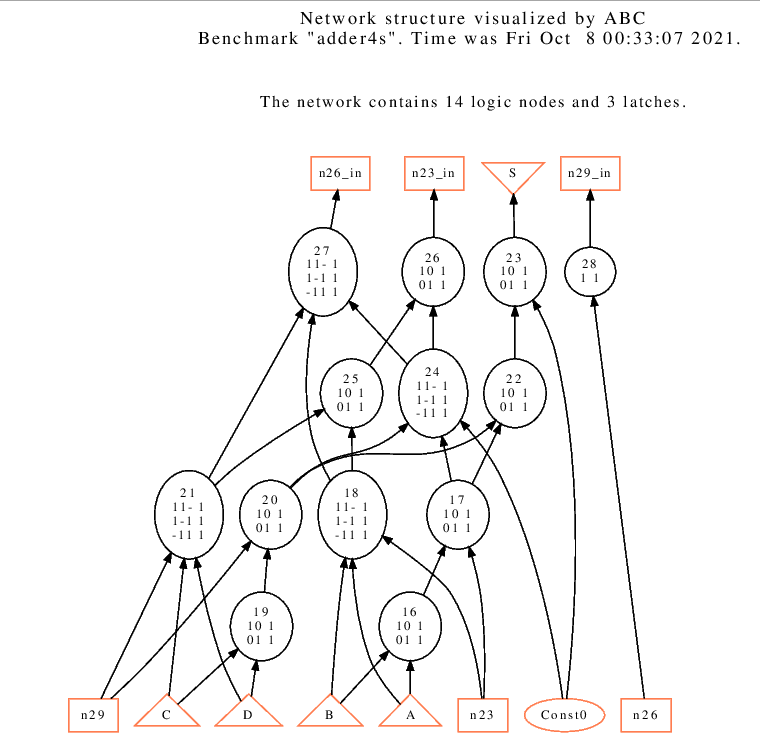
\includegraphics[width=.9\textwidth]{img/blif.png}
        \caption{Original network}
        \label{fig:blif}
        \end{minipage}
    \end{figure}
    \begin{figure}[h]
        \begin{minipage}{0.99\textwidth}
        \centering
        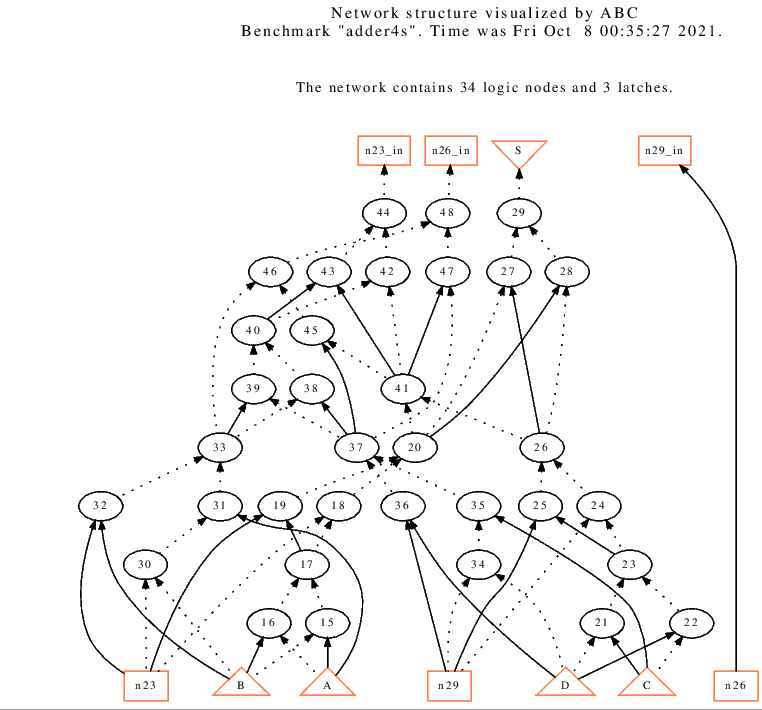
\includegraphics[width=.9\textwidth]{img/strash.png}
        \caption{Strashed network}
        \label{fig:strash}
        \end{minipage}
    \end{figure}
    \begin{figure}[h]
        \begin{minipage}{0.99\textwidth}
        \centering
        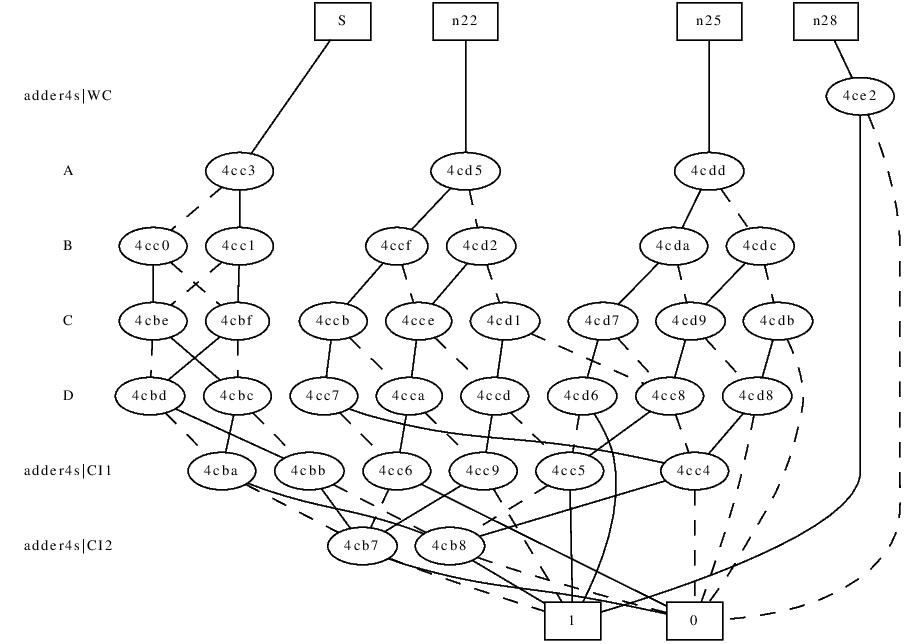
\includegraphics[width=.9\textwidth]{img/bdd.png}
        \caption{BDD of flattened network}
        \label{fig:bdd}
        \end{minipage}
    \end{figure}

    \newpage

    \section{Part 2}

    \begin{enumerate}[(a)]
        \item The difference between:
            \begin{enumerate}[1.]
                \item logic network in AIG (by command \texttt{aig}) vs. structurally hashed AIG (by command \texttt{strash})

                    The command \texttt{aig} only converts the local functions of each nodes into AIG. 
                    The nodes in the network remain the same. 
                    After the command, the command \texttt{show} will show the exact same network,
                    but the command \texttt{print\_stats} will show the number of aig nodes.

                    The command \texttt{strash} structurally hash the whole network and turn it into AIG.

                \item logic network in BDD (by command \texttt{bdd}) vs. collapsed BDD (by command \texttt{collapse}) 

                    The command \texttt{bdd} only converts the local function of each nodes into BDD.
                    The command \texttt{show\_bdd} can show the bdd of each PO.

                    The command \texttt{collapse} collapses the network,
                    resulting in one node for each PO, whose fanins are all PIs.
                    A global BDD is built and showing the BDD of a single PO is not available.

            \end{enumerate}
        \item The command \texttt{logic} transforms the AIG into a logic network with the SOP representation of the two-input AND-gates.
    \end{enumerate}
        
        
    
\end{document}
